\documentclass[10pt,landscape]{article}
\usepackage{multicol}
\usepackage{calc}
\usepackage{ifthen}
\usepackage[landscape]{geometry}
\usepackage{graphicx}
\usepackage{amsmath, amssymb, amsthm}
\usepackage{latexsym, marvosym}
\usepackage{pifont}
\usepackage{lscape}
\usepackage{graphicx}
\usepackage{array}
\usepackage{booktabs}
\usepackage[bottom]{footmisc}
\usepackage{tikz}
\usetikzlibrary{shapes}
\usepackage{pdfpages}
\usepackage{wrapfig}
\usepackage{enumitem}
\setlist[description]{leftmargin=0pt}
\usepackage{xfrac}
\usepackage{relsize}
\usepackage{rotating}


 \newcommand\independent{\protect\mathpalette{\protect\independenT}{\perp}}
    \def\independenT#1#2{\mathrel{\setbox0\hbox{$#1#2$}%
    \copy0\kern-\wd0\mkern4mu\box0}} 
            
\newcommand{\noin}{\noindent}    


\geometry{top=.4in,left=.3in,right=.4in,bottom=.4in}

\pagestyle{empty}
\makeatletter
\renewcommand{\section}{\@startsection{section}{1}{0mm}%
                                {-1ex plus -.5ex minus -.2ex}%
                                {0.5ex plus .2ex}%x
                                {\normalfont\large\bfseries}}
\renewcommand{\subsection}{\@startsection{subsection}{2}{0mm}%
                                {-1explus -.5ex minus -.2ex}%
                                {0.5ex plus .2ex}%
                                {\normalfont\normalsize\bfseries}}
\renewcommand{\subsubsection}{\@startsection{subsubsection}{3}{0mm}%
                                {-1ex plus -.5ex minus -.2ex}%
                                {1ex plus .2ex}%
                                {\normalfont\small\bfseries}}
\makeatother

\setcounter{secnumdepth}{0}

\setlength{\parindent}{0pt}
\setlength{\parskip}{0pt plus 0.5ex}

% -----------------------------------------------------------------------

\usepackage{titlesec}

\titleformat{\section}
{\color{purple}\normalfont\large\bfseries}
{\color{purple}\thesection}{1em}{}
\titleformat{\subsection}
{\color{red}\normalfont\normalsize\bfseries}
{\color{red}\thesection}{1em}{}
% Comment out the above 5 lines for black and white

\begin{document}

\raggedright
\footnotesize
\begin{multicols*}{3}

% multicol parameters
% These lengths are set only within the two main columns
%\setlength{\columnseprule}{0.25pt}
\setlength{\premulticols}{1pt}
\setlength{\postmulticols}{1pt}
\setlength{\multicolsep}{1pt}
\setlength{\columnsep}{2pt}

%%%%%%%%%%%%%%%%%%%%%%%%%%%%%%%%%%%%
%%% TITLE
%%%%%%%%%%%%%%%%%%%%%%%%%%%%%%%%%%%%

\begin{center}
    {\color{teal} \Large{\textbf{CS120 Final Cheat Sheet}}} \\
\end{center}

%%%%%%%%%%%%%%%%%%%%%%%%%%%%%%%%%%%%
%%% ATTRIBUTIONS
%%%%%%%%%%%%%%%%%%%%%%%%%%%%%%%%%%%%

\begin{center}
    Last Updated \today
\end{center}

%%%%%%%%%%%%%%%%%%%%%%%%%%%%%%%%%%%%
%%% BEGIN CHEATSHEET
%%%%%%%%%%%%%%%%%%%%%%%%%%%%%%%%%%%%


\section{Sorting Algorithms}\smallskip \hrule height 2pt \smallskip

   \subsection*{Exhaustive-Search Sort}
\textbf{Use Case:} Best for small datasets due to its exhaustive nature. Not efficient for large datasets. \\
\textbf{Algorithm 1:} Exhaustive-Search Sort
\begin{enumerate}
    \item For each permutation \( \pi : [n] \rightarrow [n] \):
    \item If \( K_{\pi(0)} \leq K_{\pi(1)} \leq \cdots \leq K_{\pi(n-1)} \):
    \item Return \( (K_{\pi(0)}, V_{\pi(0)}),(K_{\pi(1)}, V_{\pi(1)}), \ldots ,(K_{\pi(n-1)}, V_{\pi(n-1)}) \).
\end{enumerate}

\subsection*{Insertion Sort}
\textbf{Use Case:} Effective for small and partially sorted datasets. Simple implementation but inefficient for large datasets. \\
\textbf{Algorithm 2:} Insertion Sort
\begin{enumerate}
    \item For each \( i = 0, \ldots, n - 1 \):
    \item Insert \( A[i] \) into the correct place in \( (A[0], \ldots, A[i - 1]) \).
    \item Return \( A \).
\end{enumerate}

\subsection*{Merge Sort}

\textbf{Use Case:} Suitable for large datasets. Efficient and stable with a time complexity of \( O(n \log n) \), but requires additional space. \\
\textbf{Algorithm 3:} Merge Sort
\begin{enumerate}
    \item If \( n \leq 1 \) return \( A \).
    \item Else if \( n = 2 \) and \( K_0 \leq K_1 \) return \( A \).
    \item Else if \( n = 2 \) and \( K_0 > K_1 \) return \( ((K_1, V_1),(K_0, V_0)) \).
    \item Else:
Split \( A \) into two halves \( A_1 \) and \( A_2 \),  \( A_1 = \) MergeSort(first half of \( A \)),  \( A_2 = \) MergeSort(second half of \( A \)),  Return Merge(\( A_1 \), \( A_2 \)).

\end{enumerate}


\section{Computational Problems} \smallskip \hrule height 2pt \smallskip

Defined as a triple $\Pi = (I, O, f)$.
\begin{align*}
I & : \text{set of inputs/instances.} \\
O & : \text{set of outputs.} \\
f(x) & : \text{set of solutions for each } x \in I.
\end{align*}

Algorithm \( A \) solves computational problem \( \Pi = (I, O, f) \) if the following holds:
\begin{enumerate}
    \item For every input \( x \in I \) with \( f(x) \neq \emptyset \), we have \( A(x) \in f(x) \).
    \item There is a special output \( \bot \in O/ \) such that for every input \( x \in I \) with \( f(x) = \emptyset \), we have \( A(x) = \bot \).
\end{enumerate}

\section{Measuring Efficiency}

Efficiency differentiated by algorithms' efficiency.
Running time associated with input size.
Worst-case running time: $T(n) = \max$ operations on input $x$ of size $\leq n$.
$T(n)$ measures the upper bound of running time for size $n$.

\subsection{Definitions}

Given two functions \( f(n) \) and \( g(n) \), the following notations describe their growth rate relationships:

\begin{itemize}
    \item \( f = O(g) \) means \( f(n) \leq c \cdot g(n) \) for some \( c > 0 \) and sufficiently large \( n \).
    \item \( f = \Omega(g) \) means \( f(n) \geq c \cdot g(n) \) for some \( c > 0 \) and sufficiently large \( n \).
    \item \( f = \Theta(g) \) means \( f(n) \) is bounded above and below by \( g(n) \) asymptotically.
    \item \( f = o(g) \) means \( \lim_{n \to \infty} \frac{f(n)}{g(n)} = 0 \).
    \item \( f = \omega(g) \) means \( \lim_{n \to \infty} \frac{f(n)}{g(n)} = \infty \).
\end{itemize}

\textbf{Implications:}
\( o \) is a subset of \( O \) AND \( \omega \) is a subset of \( \Omega \) AND If \( f = \Theta(g) \) then \( f = o(f) \) and \( f = \omega(g) \).


\textbf{Complexity Classes Ordered from Least to Greatest:}
\( o(1) \), \( O(\log\log n) \), \( \Omega(\log n) \), \( o(n) \), \( O(n\log n) \), \( o(n^2) \), \( \Theta(n^2) \),  \( o(2^n) \),  \( \Omega(2^n) \),  \( o(n!) \),  \( \Omega(n!) \)


\subsection{Computational Complexity of Sorting}

Exhaustive-Search Sort: $\Theta(n! \cdot (n - 1))$.
Insertion Sort: $\Theta(n^2)$.
Merge Sort: $\Theta(n \log n)$.
Goal: Find algorithms with minimal growth rate for a problem $\Pi$.

\section{Reductions}\smallskip \hrule height 2pt \smallskip
\subsection{Formalism}

\textbf{Definition:}
Reduction is using one problem's solution ($\Gamma$) to solve another ($\Pi$).

\textbf{Formalism:}
If an algorithm for $\Pi$ solves $\Gamma$ using an oracle, then $\Pi$ reduces to $\Gamma$ ($\Pi \leq \Gamma$).
\textbf{Efficiency:}
If reduction runs in $O(T(n))$ time and calls an oracle once at size $h(n)$, we write $\Pi \leq_{T,h} \Gamma$.

\subsection*{Use of Reductions}

The use of reductions is mostly described by the following lemma, which we'll return to many times in CS 120:

\textbf{Lemma 3.1.} Let $\Pi$ and $\Gamma$ be computational problems such that $\Pi \leq \Gamma$. Then:
\begin{enumerate}
\item If there exists an algorithm solving $\Gamma$, then there exists an algorithm solving $\Pi$.
\item If there does not exist an algorithm solving $\Pi$, then there does not exist an algorithm solving $\Gamma$.
\item If there exists an algorithm solving $\Gamma$ with runtime $g(n)$, and $\Pi \leq_{T,h} \Gamma$, then there exists an algorithm solving $\Pi$ with runtime $O(T(n) + g(h(n)))$.
\item If there does not exist an algorithm solving $\Pi$ with runtime $O(T(n) + g(h(n)))$, and $\Pi \leq_{T,h} \Gamma$, then there does not exist an algorithm solving $\Gamma$ with runtime $O(g(n))$.
\end{enumerate}

\section{Data Structures}\smallskip \hrule height 2pt \smallskip

\subsection{Static Data Structures}

A static data structure problem is a quadruple $\Pi = (I, O, Q, f)$ where:
\begin{itemize}
\item $I$ is a (typically infinite) set of possible inputs $x$, and $O$ is a (sometimes infinite) set of possible outputs $y$.
\item $Q$ is a set of queries, and
\item For every $x \in I$ and $q \in Q$, $f(x, q) \subseteq O$ is a set of valid answers.
\end{itemize}

$Q = \{(search, K) : K \in \mathbb{R}\} \cup \{(next-smaller, K) : K \in \mathbb{R}\}$

\subsection*{Formalization}
\begin{itemize}
\item \textbf{Preprocess}$(x)$: Sort the array $x$ of key-value pairs in $O(n \log n)$ time to obtain a sorted array $x_0 = ((K_0^0, V_0^0), \ldots, (K_0^{n-1}, V_0^{n-1}))$.

\item \textbf{Eval}$(x_0, (\text{search}, K))$: Use binary search to find $i \in [n]$ such that $K_0^i = K$ in time $O(\log n)$ and return $(K_0^i, V_0^i)$. If no such $i$ exists, return $\bot$.

\item \textbf{Eval}$(x_0, (\text{next-smaller}, K))$: Use binary search to find $i = \max\{j : K_0^j < K\}$ in time $O(\log n)$ and return $(K_0^i, V_0^i)$. If no such $i$ exists (namely, if $K_0^0 \geq K$), return $\bot$.
\end{itemize}

\textbf{Theorem 5.3.} Static Predecessors has an implementation in which
\begin{itemize}
\item \textbf{Eval}$(x_0, (\text{search}, K))$ and \textbf{Eval}$(x_0, (\text{next-smaller}, K))$ both take time $O(\log n)$
\item \textbf{Preprocess}$(x)$ takes time $O(n \log n)$
\item \textbf{Preprocess}$(x)$ has size $O(n)$
\end{itemize}

\subsection{Dynamic Data Structures}
A dynamic data structure problem is a quintuple $\Pi = (I, O, U, Q, f)$ where:
\begin{itemize}
\item $I$ is a (sometimes infinite) set of possible initial inputs $x$, and $O$ is a (sometimes infinite) set of possible outputs $y$.
\item $U$ is a set of updates,
\item $Q$ is a set of queries, and
\item For every $x \in I$, $u_0, u_1, \ldots, u_{m-1} \in U$, and $q \in Q$, $f(x, u_0, \ldots, u_{m-1}, q) \subseteq O$ is a set of valid answers.
\end{itemize}

Often we take $I = \emptyset$, since the inputs can usually be constructed through a sequence of updates.

\subsubsection{Implementation}


For a dynamic data structure problem \( \Pi = (I, O, Q, U, f) \), an implementation is a triple of algorithms \( (\text{Preprocess}, \text{EvalQ}, \text{EvalU}) \) such that for all \( x \in I \), \( u_0, u_1, \ldots, u_{m-1} \in U \) and \( q \in Q \), if \( f(x, u_0, u_1, \ldots, u_{m-1}) \neq \emptyset \), we have:
\begin{align*}
\text{EvalQ}&\left(\text{EvalU}\left(\ldots \text{EvalU}\left(\text{EvalU}\left(\text{Preprocess}(x), u_0\right), u_1\right), \ldots, u_{m-1}\right), q\right) \\
&\in f(x, u_0, u_1, \ldots, u_{m-1}, q),
\end{align*}
else
\begin{align*}
\text{EvalQ}&\left(\text{EvalU}\left(\ldots \text{EvalU}\left(\text{EvalU}\left(\text{Preprocess}(x), u_0\right), u_1\right), \ldots, u_{m-1}\right), q\right) \\
&= \bot.
\end{align*}

\section{Binary Search Tree}\smallskip \hrule height 2pt \smallskip

\subsubsection{Definition}

A binary search tree (BST) is a recursive data structure. Every nonempty BST has a root vertex $r$, and every vertex $v$ has: a key $K_v$, a value $V_v$, a pointer to a left child $v_L$, which is another binary tree (possibly None, the empty BST), a pointer to a right child $v_R$, which is another binary tree (possibly None, the empty BST).

Crucially, we also require that the keys satisfy the BST Property:
\begin{itemize}
\item If $v$ has a left-child $v_L$, then the keys of $v_L$ and all its descendants are no larger than $K_v$.
\item Similarly, if $v$ has a right-child $v_R$, then the keys of $v_R$ and all of its descendants are no smaller than $K_v$.
\end{itemize}

Note that the empty set satisfies all the properties above and is a BST.

\textbf{Theorem 2.2:}
Given a binary search tree of height (equivalently, depth) $h$, all of the dynamic predecessors operations (queries and updates) can be performed in time $O(h)$.

\textbf{Definition of height:}
The height h of a BST is the length of the longest path from
the root vertex to any leaf node. The height of an empty tree is -1.

\subsection{Balanced Binary Search Trees}

\subsubsection{Definition (AVL Trees)}

An AVL Tree is a binary search tree in which:
\begin{itemize}
\item Every vertex has an additional attribute containing its height in the tree (length of the longest path from the vertex to a leaf). (``data structure augmentation'')
\item Every pair of siblings in the tree has heights differing by at most 1 (where we define the height of an empty subtree to be -1). (``height-balanced'')
\end{itemize}

\textbf{Lemma 3.2:}
Every AVL Tree with $n$ vertices has height (=depth) at most $2 \log_2 n$.

\subsubsection{Rotations on Tree}

On the left: all keys in $A$ are $\leq K_x$, all keys in $B$ are $\in [K_x, K_y]$, and all keys in $C$ are $\geq K_y \Rightarrow$ BST property is preserved on the right.

From left to right, we have the operation $Left.rotate(x)$. From right to left, we have the operation $Right.rotate(y)$.

\textbf{How much time does a rotation take?}
Rotations only take $O(1)$ time! One only needs to change a constant number of pointers – there is no traversing or other expensive operations.

\textbf{Theorem 3.3:}

We can insert a new key-value pair into an AVL Tree while preserving the AVL Tree property in time $O(\log n)$.

\section{The RAM Model}\smallskip \hrule height 2pt \smallskip

\subsubsection{RAM Program (Syntax)}

A RAM Program \( P \) is defined by variables \( V \) and commands \( C_0, C_1, \ldots, C_{`-1} \). It includes:

\begin{itemize}
    \item Assignments \( var = c \) for \( var \in V \) and \( c \in \mathbb{N} \).
    \item Arithmetic \( var_0 = var_1 \, op \, var_2 \) with \( op \in \{+, -, \times, /\} \).
    \item Memory operations \( var_0 = M[var_1] \) and \( M[var_0] = var_1 \).
    \item Conditional branching IF \( var == 0 \), GOTO \( k \).
\end{itemize}

Each program must have special variables \( input\_len \), \( output\_ptr \), and \( output\_len \).


\subsubsection*{Definition (Computation of a RAM Program: Semantics)}

A RAM Program \( P = (V, (C_0, \ldots, C_{\ell-1})) \) processes input \( x \) as follows:

\textbf{Initialization:} Encode \( x \) into natural numbers in memory \( M[0] \) to \( M[n-1] \), set \( input\_len = n \), and initialize other variables and memory to 0.

\textbf{Execution:} Follow commands \( C_0, C_1, \ldots \), executing operations, with jumps as directed by GOTO, treating negative results as 0 and rounding down divisions.

\textbf{Output:} On reaching line \( \ell \), \( P(x) \) is the memory slice from \( M[output\_ptr] \) to \( M[output\_ptr + output\_len - 1] \).

The running time \( Time_P(x) \) is the count of commands executed.


\subsubsection{Data}
In the RAM model, all inputs and outputs are arrays of natural numbers. How can we represent other types of data?


\textbf{(Signed) Integers:} Natural numbers with an additional sign bit.


\textbf{Rational Numbers:} Pairs of integers (numerator and denominator).


\textbf{Real Numbers:} Impossible! The set of real numbers is uncountable, but the set of finite sequences of natural numbers is countable. Although this is a constraint on expressivity, the inability to represent and manipulate infinite-precision real numbers is generally accepted as part of both the intuitive and physically realizable concepts of computation.


\textbf{Strings:} An array of ASCII values, where each character is represented as a number in $\{0, 1, \ldots, 127\}$.


\section{RAM and Word-RAM Simulations}\smallskip \hrule height 2pt \smallskip

\textbf{Theorem 4.1.}
For every mod-extended RAM program \( P \) that allows the modulus operation (\%), there exists an equivalent standard RAM program \( P' \) such that for any input \( x \), \( P' \) halts on \( x \) if and only if \( P \) halts on \( x \), and if they halt, \( P'(x) = P(x) \). Additionally, the runtime of \( P' \) on \( x \) is at most three times that of \( P \) on \( x \).

\textbf{Proof.}
Consider a mod operation in the extended RAM model: \( \text{var0} = \text{var1}\% \text{var2} \). This can be replaced with a sequence of operations using a temporary variable \( \text{temp} \):
\begin{enumerate}
    \item \( \text{temp} = \text{var1} / \text{var2} \)
    \item \( \text{temp} = \text{temp} \times \text{var2} \)
    \item \( \text{var0} = \text{var1} - \text{temp} \)
\end{enumerate}
The threefold increase in operations results in a runtime of \( P' \) on \( x \), denoted \( T_{P'}(x) \), being at most three times \( T_{P}(x) \), which falls within the \( O(\cdot) \) notation. Consequently, the inclusion of the mod operation does not affect the asymptotic runtime growth rate.

\subsection{WORD RAM Model}

The Word RAM Model is defined like the RAM Model, except that it has a dynamic word length $w$ and memory size $S$ that are used as follows:

\begin{itemize}
\item \textbf{Memory:} An array of length $S$, with entries in $\{0, 1, \ldots, 2^{w-1}\}$. Reads and writes to memory locations larger than $S$ have no effect.
\item \textbf{Operations:} Addition and multiplication are redefined from the RAM Model to return $2^w - 1$ if the result would be $\geq 2^w$.
\item \textbf{Initial Settings:} When a computation is started on an input $x$, which is an array consisting of $n$ natural numbers, the memory size is taken to be $S = n$, and word length is taken to be $w = \lfloor \log \max\{S, x[0], \ldots, x[n-1]\} \rfloor + 1$. This setting is to ensure that $S, x[0], \ldots, x[n-1]$ are all strictly smaller than $2^w$ and hence fit in one word.
\item \textbf{Increasing $S$ and $w$:} If the algorithm needs to increase its memory size beyond $S$, it can issue a MALLOC command, which increments $S$ by 1, sets $M[S - 1] = 0$, and if $S = 2^w$, it also increments $w$ by 1.
\end{itemize}

\subsubsection{WORD RAM vs RAM Model}

A. For every RAM program $P$, there is a Word-RAM Program $P_0$ such that $P_0$ halts on $x$ iff $P$ halts on $x$, and if they halt, then $P_0(x) = P(x)$ and $T_{P_0}(x) = O\left((T_P(x) + n + S) \cdot \left(\log M_{w_0}\right)^{O(1)}\right)$, where $n$ is the length of the input $x$, $S$ is the largest memory location accessed by $P$ on input $x$, $M$ is the largest number computed by $P$ on input $x$, and $w_0 = \lfloor \log \max\{n, x[0], \ldots, x[n-1]\} \rfloor + 1$.

\textbf{Proof:}
We need to be able to simulate anything RAM does that Word RAM doesn't. This means we need to replace each number stored by \( P \) using a linked list bignum representation with the word length at the time the number was stored. We also need to periodically use \texttt{MALLOC} to ensure that memory remains large enough to hold all of \( P \)'s associated memory -- this costs \( O(S) \) and for bignum representations, which yield an \( O(\log M / \log w) \) blowup because it upper bounds the number of digits needed to represent numbers from \( M \) in base \( 2^w \).


B.  For every Word-RAM program $P$, there is a RAM program $P_0$ such that $P_0$ halts on $x$ iff $P$ halts on $x$, and if they halt, then $P_0(x) = P(x)$ and $T_{P_0}(x) = O(T_P(x) + n + w_0)$, where $n$ is the length of $x$ and $w_0$ is the initial word size of $P$ on input $x$.

\textbf{Proof:}
We need to calculate the memory size (initially \( = \) input length) and word length (initially through \( O(n) \) max operation and \( O(w) \) log operations). Temporary variable \( \text{max-num} = 2^w \) can be calculated in \( O(w) \) time.

Memory modification: do nothing for \( M[i] \) commands if \( i \) is greater than \( \text{mem-size} \). Addition and multiplication need to be clamped. Adjust \( \text{GOTO} \) line numbers.

\texttt{MALLOC}: Check if \( \text{mem-size} \geq 2^w \) (through subtraction). If not, increment \( \text{mem-size} \) by 1, \( \text{word-len} \) by 1, and \( \text{max-num} \) by \( *= 2 \).


\section{Randomized Algorithms and Data Structures}\smallskip \hrule height 2pt \smallskip

\subsubsection*{Las Vegas Algorithms}

Las Vegas Algorithms are algorithms that always output a correct answer, but their running time depends on their random choices. Worst case, infinite RT. Typically, We say the (worst-case) expected running time of algorithm $A$ is given by:

\[
T(n) = \max_{x: \text{size}(x) \leq n} \mathbb{E}[T_A(x)],
\]

where $T_A(x)$ is the random variable denoting the runtime of algorithm $A$ on input $x$, and $\mathbb{E}[\cdot]$ denotes the expectation of a random variable.

\textbf{EXAMPLE 1.) Input:} A composite number $n$

\textbf{Output:} A number $k < n$ that divides $n$.

The computational problem is called "Factorize," and a Las Vegas algorithm for it is as follows:
\texttt{Factorize}(n), repeat = 1, sqrt = $\sqrt{n}$, while repeat = 1 do, p = random(sqrt), if p divides n then (repeat = 0 and return p).

The algorithm correctly solves the computational problem, and its expected runtime is $O(\sqrt{n})$.

\subsubsection*{Monte Carlo Algorithms}

Monte Carlo Algorithms are algorithms that always run within a desired time bound $T(n)$ but may err with some small probability (if they are unlucky in their random choices). In other words, we say that algorithm $A$ solves computational problem $\Pi = (I, O, f)$ with error probability $p$ if the following conditions hold:

\begin{enumerate}
\item For every $x \in I$ such that $f(x) \neq \emptyset$, $\Pr[A(x) \in f(x)] \geq 1 - p$.
\item For every $x \in I$ such that $f(x) = \emptyset$, $\Pr[A(x) = \bot] \geq 1 - p$.
\end{enumerate}

COND 1 ensure that when  algorithm produces output for inputs with non-empty solutions, it is correct with high probability. COND 2 guarantees that when the algorithm produces no output (indicated by $\bot$) for inputs with empty solutions, it does so with high probability.

\subsubsection{Which is preferable (Las Vegas or Monte Carlo)?}
Las Vegas. Las Vegas algorithm can be converted into a Monte Carlo, not other way. It can be easier to come up with Monte Carlo algorithms. 

\subsection{QuickSelect}
\begin{itemize}
\item Randomized algorithm for selecting the k-th smallest (or largest) element from an unsorted list.
\item Efficiently solves the Selection problem, Similar to QuickSort in partitioning.
\item Recursively focuses on one partition, leading to expected linear time complexity of $O(n)$.
\item Worst-case time complexity can be $O(n^2)$, but it's unlikely with random pivot selection.

\end{itemize}


\section{Dictionaries and Graphs}\smallskip \hrule height 2pt \smallskip
\subsubsection*{Monte Carlo Data Structure}

\begin{itemize}
\item \textbf{Preprocess(U, m):} Initialize an array $A$ of size $m$. In addition, choose a random hash function $h : [U] \to [m]$ from the universe $[U]$ to $[m]$.

\item \textbf{Insert(K, V):} Place $(K, V)$ into the linked list at slot $A[h(K)]$.

\item \textbf{Delete(K):} Remove an element from the linked list at slot $A[h(K)]$.

\item \textbf{Search(K):} Return the head of the linked list at $A[h(K)]$.

\end{itemize}

\subsubsection*{Las Vegas Data Structure (Hash Table)}

This data structure is similar to the one mentioned earlier, but with a different Search operation:

\begin{itemize}
\item \textbf{Preprocess(U, m):} Initialize an array $A$ of size $m$. Also, choose a random hash function $h : [U] \to [m]$ from the universe $[U]$ to $[m]$.

\item \textbf{Insert(K, V):} Place $(K, V)$ into the linked list at slot $A[h(K)]$.

\item \textbf{Delete(K):} Remove an element from the linked list at slot $A[h(K)]$.

\item \textbf{Search(K):} Walk through the linked list at $A[h(K)]$ and return the first element with the correct key $K$ (returning $\bot$ if none is found).

\end{itemize}

In this Las Vegas data structure, we bound the expected runtime in a similar way as before. The additional linked list checking adds only an $O(1)$ slowdown if there are no collisions among elements. The expected runtime is $O(1 + \frac{n}{m})$, where $\alpha = \frac{n}{m}$ is the load of the table.

\subsubsection{Shortest Walks}

Let $G = (V, E)$ be a directed graph, and $s, t \in V$.

- A walk $w$ from $s$ to $t$ in $G$ is a sequence $v_0, v_1, \ldots, v'$ of vertices such that $v_0 = s$, $v' = t$, and $(v_{i-1}, v_i) \in E$ for $i = 1, \ldots, '$.

- The length of a walk $w$ is denoted as $\text{length}(w)$, which is the number of edges in $w$ (i.e., the number $'$ above).

- The distance from $s$ to $t$ in $G$ is defined as:
  \[
  \text{dist}_G(s, t) = \begin{cases}
  \min\{\text{length}(w) : w \text{ is a walk from } s \text{ to } t\} & \text{if $\exists$ walk} \\
  \infty & \text{otherwise}
  \end{cases}
  \]

- A shortest walk from $s$ to $t$ in $G$ is a walk $w$ from $s$ to $t$ with $\text{length}(w) = \text{dist}_G(s, t)$.

\textbf{Lemma 3.2.} If $w$ is a shortest walk from $s$ to $t$, then all of the vertices that occur on $w$ are distinct.

\subsubsection{Breadth-First Search}

BFS is graph traversal algorithm used to explore and analyze the structure of a graph or tree. It systematically visits all the vertices of a graph, starting from a specified source vertex, and proceeds by visiting vertices level by level, i.e., it explores all vertices at distance 1 from the source, then all vertices at distance 2, and so on.

\textbf{Theorem 5.2.} BFS($G$) correctly solves DistanceInGraph and can be implemented in time $O(n+m)$, where $n$ is the number of vertices in $G$ and $m$ is the number of edges.

\subsection{Graph Coloring}

For an undirected graph $G = (V, E)$, a \textit{(proper) k-coloring} of $G$ is a mapping
$f : V \to [k]$ such that for all edges $\{u, v\} \in E$, we have $f(u) \neq f(v)$.
An improper coloring allows us to assign the same color to vertices that share an edge, but we
will work with proper colorings unless we explicitly state otherwise.

\subsubsection{Greedy Coloring}
The Greedy Coloring algorithm takes a graph and assigns colors to each vertex such that no two adjacent vertices (vertices connected by an edge) have the same color. The goal is to use as few colors as possible. Here's a step-by-step explanation:

\begin{enumerate}
\item First, take a graph, which is just a collection of points called vertices, connected by lines called edges.
\item Now, create a list of all the vertices in some order. It doesn't have to be in any specific order, just any sequence of all the vertices.
\item Then, go through each vertex one by one, according to the order you listed them.
\item For each vertex, choose the smallest number that hasn't been used by its neighboring vertices. Think of each number as a different color. CONTINUE this
\end{enumerate}


\textbf{Theorem 4.1: }When run on a graph $G = (V, E)$ with any ordering of vertices, Greedy Coloring ($G$) will use at most $d_{\text{max}} + 1$ colors, where $d_{\text{max}} = \max\{d(v) : v \in V\}$.

\textbf{Corollary 4.3}Graph 2-Coloring can be solved in time $O(n + m)$.

\begin{proof}
We can partition $G$ into connected components in time $O(n+m)$. Then, for each connected component, we can use BFSColoring on each component, which takes a total time of $O(n + m)$.
\end{proof}

\textbf{Theorem 2.1.} If $G$ is a connected 2-colorable graph, then BFSColoring($G$) will color $G$ using 2 colors.


\section{Independent Sets, Interval Scheduling, Matchings}\smallskip \hrule height 2pt \smallskip
\textbf{Independent Set:}

Let $G = (V, E)$ be a graph. An independent set in $G$ is a subset $S \subseteq V$ such that there are no edges entirely in $S$. That is, $\{u, v\} \in E$ implies that $u \notin S$ or $v \notin S$.

A proper $k$-coloring of a graph $G$ is equivalent to a partition of $V$ into $k$ independent sets (each color class should be an independent set).

When we have a graph $G = (V, E)$ representing conflicts, instead of partitioning $V$ into a small number of conflict-free subsets (as coloring would), it is sometimes useful to instead find a single, large conflict-free subset. This gives rise to the following computational problem:

\textbf{Independent Set Problem:}

\textit{Input:} A graph $G = (V, E)$

\textit{Output:} An independent set $S \subseteq V$ in $G$ of maximum size

\subsubsection{Theorem 3.2.} For every graph $G$ with $n$ vertices and $m$ edges, GreedyIndSet($G$) can be implemented in time $O(n + m)$ and outputs an independent set of size at least $\frac{n}{d_{\text{max}} + 1}$, where $d_{\text{max}}$ is the maximum vertex degree in $G$.

\textbf{Theorem 3.3.} If the input intervals are sorted by increasing order of end time $b_i$, then we have that GreedyIntervalScheduling($x$) will find an optimal solution to IntervalScheduling-Optimization, and can be implemented in time $O(n \log n)$.

\subsection{Matchings}
\textbf{Definition 3.1.} For a graph $G = (V, E)$, a matching in $G$ is a subset $M \subseteq E$ such that every vertex $v \in V$ is incident to at most one edge in $M$. Equivalently, no two edges in $M$ share an endpoint.

\smallskip 
Maximum Matching can be viewed as a special case of the Independent Set problem we studied last time. There's an efficient reduction from Maximum Matching to Independent Set. In Maximum Matching, we aim to find a set of non-conflicting edges, while Independent Set seeks non-conflicting vertices. Thus, let $V_0 = E$ and $E_0 = \{\{e, e_0\} : e, e_0$ share an endpoint\}. The graph $G_0$ is known as the line graph of $G$. Unfortunately, the fastest known algorithm for Independent Set runs in approximately $O(1.2^n)$. However, special cases of Independent Set, like Matching, can be solved more quickly.

\textbf{Definition 5.1.} Let $G = (V, E)$ be a graph, and $M$ be a matching in $G$. Then:
\begin{enumerate}
\item An alternating walk $W$ in $G$ with respect to $M$ is a walk $(v_0, v_1, \ldots, v^\prime)$ in $G$ such that for every $i = 1, \ldots, \ell - 1$, $\{v_{i-1}, v_i\} \in M \Leftrightarrow \{v_i, v_{i+1}\} \in E \setminus M$.
\item An augmenting path $P$ in $G$ with respect to $M$ is an alternating walk in which $v_0$ and $v^\prime$ are respectively unmatched by $M$, and in which all of the vertices in the walk are distinct, and $\ell \geq 1$.
\end{enumerate}

For example, consider the following graph with $M = \{\{1, C\}, \{3, F\}, \{5, A\}\}$.
We check whether the following sequences of vertices constitute an alternating walk or an augmenting path.

\begin{minipage}{\linewidth}
            \centering
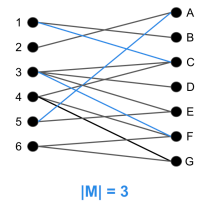
\includegraphics[width=1.5in]{figures/graph.png}
        \end{minipage}

\begin{center}
\begin{tabular}{|c|c|c|}
\hline
Path & Alternating Walk & Augmenting Path \\
\hline
$2, A, 5$ & Yes & No \\
$G, 4$ & Yes & Yes \\
$3, F, 4, C, 3$ & No & N/A \\
$1, C, 6$ & No & N/A \\
$6, F, 3, C, 1, B$ & Yes & Yes \\
\hline
\end{tabular}
\end{center}

\textbf{Lemma 5.2.} Given a graph $G = (V, E)$, a matching $M$, and an augmenting path $P$ with respect to $M$, we can construct a matching $M_0$ with $|M_0| = |M| + 1$ in time $O(n)$.

\smallskip

\textbf{Definition 5.3.} A graph $G = (V, E)$ is bipartite if it is 2-colorable. That is, there is a partition of vertices $V = V_0 \cup V_1$ (with $V_0 \cap V_1 = \emptyset$) such that all edges in $E$ have one endpoint in $V_0$ and one endpoint in $V_1$.

\smallskip

\textbf{Theorem 5.4 (Berge's Theorem).} Let $G = (V, E)$ be a graph, and $M \subseteq E$ be a matching. If (and only if) $M$ is not a maximum-size matching, then $G$ has an augmenting path with respect to $M$.

\smallskip

\textbf{Lemma 5.5.} Let $G = (V_0 \cup V_1, E)$ be bipartite and let $M$ be a matching in $G$ that is not of maximum size. Let $U$ be the vertices that are not matched by $M$, and $U_0 = V_0 \cap U$ and $U_1 = V_1 \cap U$. Then:
1. $G$ has an alternating walk with respect to $M$ that starts in $U_0$ and ends in $U_1$.
2. Every shortest alternating walk from $U_0$ to $U_1$ is an augmenting path.

\smallskip

\textbf{Theorem 5.6.} Maximum Matching can be solved in time $O(mn)$ on bipartite graphs with $m$ edges and $n$ vertices.

\section{Logic}\smallskip \hrule height 2pt \smallskip

\begin{itemize}
    \item A \textit{literal} is a variable (e.g., $x_i$) or its negation ($\neg x_i$).
    \item A boolean formula is in \textit{conjunctive normal form (CNF)} if it is the AND of a sequence of \textit{clauses}, each of which is the OR of a sequence of \textit{literals}.
    \item It will be convenient to also allow 1 (true) to be a clause. 0 (false) is already a clause: the empty clause is always false.
\end{itemize}


\textbf{Definition 2.1 (informal).} A boolean formula $\phi$ is a formula built up from a finite set of variables, say $x_0, \ldots, x_{n-1}$, using the logical operators $\land$ (AND), $\lor$ (OR), and $\neg$ (NOT), and parentheses. Every boolean formula $\phi$ on $n$ variables defines a boolean function, which we'll abuse notation and also denote by $\phi : \{0, 1\}^n \to \{0, 1\}$, where we interpret $0$ as false and $1$ as true, and give $\land$, $\lor$, $\neg$ their usual semantics (meaning).

\smallskip

\textbf{Definition 2.2.} A literal is a variable (e.g., $x_i$) or its negation ($\neg x_i$).

A boolean formula is in disjunctive normal form (DNF) if it is the OR of a sequence of terms, each of which is the AND of a sequence of literals.

A boolean formula is in conjunctive normal form (CNF) if it is the AND of a sequence of clauses, each of which is the OR of a sequence of literals.

\smallskip

\textbf{Lemma 2.3.} Any boolean function $f : \{0, 1\}^n \to \{0, 1\}$ can be represented by equivalent DNF and CNF formulas $\phi$ and $\psi$, respectively.

\textbf{Proof.} Construct DNF $\phi$ by OR-ing terms representing satisfying inputs of the function, with each term being an AND of input variables or their negations. Similarly, CNF $\psi$ is constructed by AND-ing clauses representing non-satisfying inputs, with each clause being an OR of variables or their negations. These constructions ensure the equivalence of $f$ with both $\phi$ and $\psi$, although they may not yield the smallest formulas.

\subsubsection{Modelling w Satisfiability}

\textbf{Theorem 4.1.} Graph k-Coloring on graphs with $n$ nodes and $m$ edges can be reduced in time $O(n + km)$ to SAT on CNF formulas with $kn$ variables and $n + km$ clauses.

\textbf{Claim 4.2:} If $G$ has a valid $k$-coloring, $\varphi_G$ is satisfiable. \\
$\Rightarrow$ We won't incorrectly output $\bot$.

\textbf{Claim 4.3:} If $\alpha$ satisfies $\varphi_G$, then $f_\alpha$ is a proper $k$-coloring of $G$. \\
$\Rightarrow$ If we output a coloring, it will be proper.

\section{Satisfiability and Solving 2-SAT}\smallskip \hrule height 2pt \smallskip

\textbf{Theorem 3.1.} There is an algorithm that solves the computational problem 2-SAT in time $O(nm)$, where $n$ is the number of variables and $m$ is the number of clauses.

At the heart of this theorem is the construction of a digraph for the CNF formula $\phi$, which allows us to use some of the graph algorithms we have already seen. The edges in this digraph capture 'implications' in the CNF formula.

\textbf{Example:} Consider the CNF formula $\phi_1$ given by
\[
\phi_1 = (\neg x_0 \lor x_1) \land (\neg x_1 \lor x_2) \land (\neg x_2 \lor x_3) \land (\neg x_3 \lor x_0).
\]

The CNF formula $(\neg a \lor \neg b)$ can be represented as shown in Figure 1:

\begin{minipage}{\linewidth}
            \centering
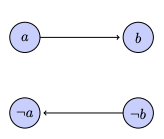
\includegraphics[width=1.3in]{figures/graph1.png}
        \end{minipage}


$\phi_1$ can also be represented as a chain of implications, as shown in Figure 2:

\begin{minipage}{\linewidth}
            \centering
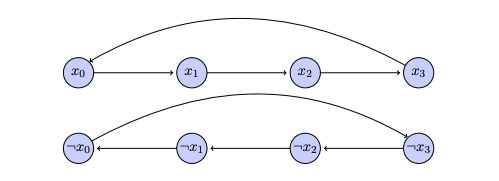
\includegraphics[width=3.5in]{figures/graph2.png}
        \end{minipage}

The CNF $\phi_1$ is satisfiable with the assignments $(1, 1, 1, 1)$ and $(0, 0, 0, 0)$.

\smallskip

\textbf{Theorem 3.2.} There is an algorithm that solves the computational problem 2-SAT-Decision in
time $O(nm)$, where $n$ is the number of variables and $m$ is the number of clauses.

\textbf{Theorem 3.3.} A CNF formula $\phi$ in which each clause has width 2 is satisfiable iff for any variable $x_i$, there is no path from $x_i$ to $\neg x_i$ AND no path from $\neg x_i$ to $x_i$ in the implication digraph $G$.

In other words, as long as there are no bad cycles of the type shown in Figure 4, the CNF formula is satisfiable. Theorem 3.3 gives the following reduction from the problem 2SAT-Decision.

\subsection{The Church-Turing Thesis}

\textbf{Theorem 4.1 (Turing-equivalent models).} If a computational problem $\Pi$ is solvable in one of the following models of computation: RAM programs, Word-RAM programs, XOR-extended RAM or Word-RAM programs, extended RAM or Word-RAM programs, Python programs, $\ldots$, then it is solvable in all of them. Moreover, there is an algorithm (e.g., a RAM program) that can transform a program in any of these models of computation into an equivalent program in any of the others.

\smallskip

\textbf{The Church–Turing Thesis:} The equivalence of many disparate models of computation leads to the Church–Turing Thesis, which has (at least) two different variants:
\begin{enumerate}
  \item The (equivalent) models of computation in Theorem 4.1 capture our intuitive notion of an algorithm.
  \item Every physically realizable computation can be simulated by one of the models in Theorem 4.1.
\end{enumerate}
This is not a precise mathematical claim, and thus cannot be formally proven, but it has stood the test of time very well, even in the face of novel technologies like quantum computers (which have yet to be built in a scalable fashion); every problem that can be solved by a quantum algorithm can also be solved by a RAM program, albeit much more slowly.

\section{Computational Complexity}\smallskip \hrule height 2pt \smallskip

To develop a robust and clean theory for classifying problems according to computational complexity, we make two choices:
\begin{itemize}
  \item A problem-independent size measure. Recall that we allowed ourselves to use different size parameters for different problems (array length $n$ and universe size $U$ for sorting; number $n$ of vertices and number $m$ of edges for graphs, number $n$ of variables and number $m$ of clauses for Satisfiability). To classify problems, it is convenient to simply measure the size of the input by its length $N$ in bits. For example:
    \begin{itemize}
      \item Array of $n$ numbers from universe size $U$: $N = \Theta(n \log_2 U)$.
      \item Graphs on $n$ vertices and $m$ edges in adjacency list notation: $N = \Theta((n + m) \log n)$.
      \item 3-SAT formulas with $n$ variables and $m$ clauses: $N = \Theta(m \log n)$.
    \end{itemize}
  \item Polynomial slackness in running time: We will only try to make coarse distinctions in running time, e.g. polynomial time vs. super-polynomial time. If the Extended Church-Turing Thesis is correct, the theory we develop will be independent of changes in computing technology. It is possible to make finer distinctions, like linear vs. nearly linear vs. quadratic, if we fix a model (like the Word-RAM), and a newer subfield called Fine-Grained Complexity does this.
\end{itemize}

\subsubsection{Definition 2.1}
\begin{itemize}
  \item For a function $T : \mathbb{N} \rightarrow \mathbb{R}^+$, $\text{TIME}_{\text{search}}(T(N))$ is the class of computational problems $\Pi = (I, O, f)$ such that there is a Word-RAM program solving $\Pi$ in time $O(T(N))$ on inputs of bit-length $N$.
  $\text{TIME}(T(N))$ is the class of decision (i.e., yes/no) problems in $\text{TIME}_{\text{search}}(T(N))$.
  \item (Polynomial time) $\text{P}_{\text{search}} = \bigcup_c \text{TIME}_{\text{search}}(n^c)$, $\text{P} = \bigcup_c \text{TIME}(n^c)$.
  \item (Exponential time) $\text{EXP}_{\text{search}} = \bigcup_c \text{TIME}_{\text{search}}(2^{n^c})$, $\text{EXP} = \bigcup_c \text{TIME}(2^{n^c})$.
\end{itemize}

\textbf{Definition 2.3}
$\mathbf{\Pi}$ and $\mathbf{\Gamma}$, we write $\mathbf{\Pi \leq_p \Gamma}$ if there is a polynomial-time reduction $\mathbf{R}$ from $\mathbf{\Pi}$ to $\mathbf{\Gamma}$. That is, there should exist $\mathbf{c \in \mathbb{R}}$ such that on an input of length $\mathbf{N}$, the reduction runs in time $\mathbf{O(N^{c})}$, if we count the oracle calls as one time step (as usual).

\smallskip

\textbf{Lemma 2.4.} Let $\Pi$ and $\Gamma$ be computational problems such that $\Pi \leq_p \Gamma$. Then:
\begin{enumerate}
  \item If $\Gamma \in \text{Psearch}$, then $\Pi \in \text{Psearch}$.
  \item If $\Pi \notin \text{Psearch}$, then $\Gamma \notin \text{Psearch}$.
\end{enumerate}

\textbf{Procedure for Proving That Problems Are Not in $\text{Psearch}$:}

\begin{enumerate}
  \item Identify a particular problem $\Pi$ in $\text{EXPsearch} \setminus \text{Psearch}$. One example is deciding whether a Word-RAM program halts within $2^n$ steps on an input $x$ of length $n$.
  \item Show that $\Pi$ reduces to the problems you are interested in, via a polynomial-time reduction.
\end{enumerate}


\smallskip

\textbf{Lemma 2.5.} We can compose reductions - if $\Pi \leq_p \Gamma$ and $\Gamma \leq_p \Theta$ then $\Pi \leq_p \Theta$.

\section{NP and NP-completeness}\smallskip \hrule height 2pt \smallskip

\textbf{Definition 3.1.} A computational problem $\Pi = (I, O, f)$ is in NPsearch if the following conditions hold:
\begin{enumerate}
  \item All solutions are of polynomial length: There is a polynomial $p$ such that for every $x \in I$ and every $y \in f(x)$, we have $|y| \leq p(|x|)$, where $|z|$ denotes the bit length of $z$.
  \item All solutions are verifiable in polynomial time: There exists a polynomial-time verifier $V$ that, given $x \in I$ and a potential solution $y$, decides whether $y \in f(x)$.
\end{enumerate}

(Remark on terminology: NPsearch is often called FNP in the literature, and is closely related to, but slightly more restricted than, the class PolyCheck defined in the MacCormick text.)

\textbf{Definition 4.1 (NP-completeness, search version).} A problem $\Pi$ is NPsearch-complete if:
\begin{enumerate}
  \item $\Pi$ is in NPsearch.
  \item $\Pi$ is NPsearch-hard: For every computational problem $\Gamma \in$ NPsearch, $\Gamma \leq_p \Pi$.
\end{enumerate}

We can think of the NP-complete problems as the “hardest” problems in NP. Indeed:

\textbf{Proposition 4.2.} Suppose $\Pi$ is NPsearch-complete. Then $\Pi \in$ Psearch if and only if NPsearch $\subseteq$ Psearch.

Remarkably, there are natural NP-complete problems. The first one is CNF-Satisfiability:

\subsubsection{Theorem 4.3 (Cook–Levin Theorem).} SAT is NPsearch-complete.

\smallskip

\textbf{Theorem 5.1.} 3-SAT is NPsearch-complete.

\textbf{Claim 5.2.} If $\phi$ is satisfiable, then $\phi_0 = R(\phi)$ is satisfiable.

\textbf{Proof of claim.} Assume that $\phi$ is satisfiable. Let $\phi = \phi_0, \phi_1, \ldots, \phi_t = R(\phi)$ be the formula $\phi_0$ as it evolves through the $t$ loop iterations. We will prove by induction on $i$ that $\phi_i$ is satisfiable for $i = 0, \ldots, t$.

\textbf{Base case (i = 0):} $\phi_0 = \phi$, which is satisfiable by hypothesis.

\textbf{Induction step:} By the induction hypothesis, we can assume that $\phi_{i-1}$ is satisfiable, and now we need to show that $\phi_i$ is satisfiable:

Suppose $\alpha_{i-1}$ is a satisfying assignment to $\phi_{i-1}$, and we obtain $\phi_i$ from it by breaking up clause $C = (\ell_0 \lor \ldots \lor \ell_k)$. Then, since $\alpha$ satisfies $C$, it satisfies at least one of $(\ell_0 \lor \ell_1)$ and $(\ell_2 \lor \ldots \lor \ell_k)$. If it satisfies the first, we can set $y = 0$ and obtain an assignment $\alpha_i$ that satisfies both $(y \lor \ell_0 \lor \ell_1)$ and $(\neg y \lor \ell_2 \ldots \ell_{k-1})$, and hence $\phi_i$. In the second case, we can set $y = 1$. Thus, we've maintained that a satisfying assignment exists.

\subsubsection{Proving NP-search-Completeness:}

To prove that a problem \( \Gamma \) is NP-search-complete, follow these steps:

\begin{enumerate}
  \item Select a known NP-search-complete problem \( \Pi \) similar to \( \Gamma \) or default to 3-SAT.
  \item Devise a polynomial-time algorithm \( R \) that transforms instances \( x \) of \( \Pi \) to instances \( R(x) \) of \( \Gamma \), using variable and clause gadgets to reflect true/false assignments and clause satisfaction.
  \item Verify that \( R \) runs in polynomial time.
  \item Ensure solutions of \( x \) map to solutions of \( R(x) \) and vice versa.
  \item Demonstrate the transformation between \( R(x) \) and \( x \) is efficient.
\end{enumerate}

This establishes NP-search-hardness. For NP-search-completeness, additionally confirm that \( \Gamma \) belongs to NP-search.

 \textbf{Theorem 5.1.} IndependentSet is NPsearch-complete.

\subsection{The P vs. NP Problem}

\textbf{Definition 3.1.} A computational problem $\Pi = (I, O, f)$ is a decision problem if $O = \{ \text{yes}, \text{no} \}$ and for every $x \in I$, $|f(x)| = 1$. The choice of the names "yes" and "no" for the 2 elements of $O$ is arbitrary, and other common choices are $O = \{1, 0\}$ and $O = \{\text{accept}, \text{reject}\}$. But it is convenient to standardize the names, since in the definition of NP below we will treat "yes" and "no" asymmetrically.

By definition:
\[ P = \{ \Pi : \Pi \in P_{\text{search}} \text{ and } \Pi \text{ is a decision problem} \} \]
\[ \text{EXP} = \{ \Pi : \Pi \in \text{EXP}_{\text{search}} \text{ and } \Pi \text{ is a decision problem} \} \]

However, the decision class NP has a more subtle definition in terms of NP-search:

\textbf{Definition 3.2 (NP).} A decision problem $\Pi = (I, \{\text{yes}, \text{no}\}, f)$ is in NP if there is a computational problem $\Gamma = (I, O, g) \in \text{NP}_{\text{search}}$ such that for all $x \in I$, we have:
\[ f(x) = \{\text{yes}\} \Leftrightarrow g(x) \neq \emptyset \]
\[ f(x) = \{\text{no}\} \Leftrightarrow g(x) = \emptyset \]

\textbf{Lemma 3.3.} $P \subseteq NP$.

\textbf{Theorem 3.4 (Search vs. Decision).} NP = P if and only if NPsearch $\subseteq$ Psearch.

\textbf{Lemma 3.5.} Satisfiability $\leq_p$ Satisfiability-Decision

\textbf{If P = NP:}
\begin{itemize}
  \item Searching for solutions is never much harder than verifying solutions.
  \item Optimization is easy.
  \item Finding mathematical proofs (for theorems that have short mathematical proofs) is easy.
  \item Breaking cryptography is easy.
  \item Machine learning is easy.
  \item Every problem in NP is NP-complete (ps9).
\end{itemize}

\textbf{If P $\neq$ NP:}
\begin{itemize}
  \item None of the NP-complete problems have (worst-case) polynomial-time algorithms. One has to settle for superpolynomial-time algorithms, heuristics that perform well on average/real-world instances (like SAT solvers), or approximation algorithms (which don't necessarily find optimal solutions).
  \item There are problems in NP that are neither NP-hard nor in P, and similarly for search problems. Natural candidates include factoring and finding Nash Equilibria of 2-player games.
  \item There is hope for secure cryptography (but this seems to require assumptions stronger than P $\neq$ NP).
\end{itemize}

\subsection{Uncomputability by reductions}

\textbf{Theorem 2.1.}
\begin{enumerate}
  \item (Universal RAM simulator in RAM) There is a RAM program $U$ such that for every RAM program $P$ and input $x$, $U$ halts on input $(P, x)$ if and only if $P$ halts on $x$, and if so, $U(P, x) = P(x)$. Moreover, $T_U((P, x)) = O(T_P(x) + |P| + |x|)$.

  \item (Universal Word-RAM simulator in Word-RAM) There is a Word-RAM program $U$ such that for every Word-RAM program $P$ and input $x$, we have $U(P, x) = P(x)$. Moreover, $T_U((P, x)) = O(T_P(x) + |P| + |x|)$.
\end{enumerate}

\subsubsection*{The Halting Problem}

The Halting Problem centers on whether a universal program can determine if a given program $P$ halts on input $x$. Ideally, such a program, denoted as $U$, would simulate $P$ and report if $P$ would never halt on $x$. However, creating a universal simulator that accurately predicts halting without running indefinitely is impossible.

For example, a simulator $U_0$ running $P$ for a limited number of steps (like $\frac{n}{120}$) could falsely conclude that $P$ doesn't halt even when it does after more steps.

Formally, the Halting Problem is defined as:

\begin{itemize}
  \item \textbf{Input:} A RAM program $P$ and an input $x$.
  \item \textbf{Output:} "yes" if $P$ halts on $x$, "no" otherwise.
\end{itemize}

\textbf{Theorem 3.1} states that no algorithm, modeled as a RAM program, can solve the Halting Problem.

\subsubsection{Unsolvability}

\textbf{Definition 4.1.} Let $\Pi = (I, O, f)$ be a computational problem. We say that $\Pi$ is solvable if there exists an algorithm $A$ that solves $\Pi$. Otherwise, we say that $\Pi$ is unsolvable.

\textbf{Lemma 4.2.} Let $\Pi$ and $\Gamma$ be computational problems such that $\Pi \leq \Gamma$. Then:
\begin{enumerate}
  \item If $\Pi$ is unsolvable, then $\Gamma$ is unsolvable.
\end{enumerate}

\textbf{Theorem 5.1.} HaltOnEmpty is unsolvable.

\textbf{Theorem 5.3.} Solves3Coloring is unsolvable.

\subsection{Uncomputable Problems}

\textbf{Definition 2.1.} Let $\Pi = (I, \{ \text{yes}, \text{no} \}, f)$ be a decision problem, and let $P$ be a RAM program. We say that $P$ solves $\Pi$ if:

\begin{itemize}
  \item For every $w \in I$ such that $f(w) = \text{yes}$, $P(w)$ halts and returns "yes."
  \item For every $w \in I$ such that $f(w) = \text{no}$, $P(w)$ halts and returns "no."
\end{itemize}

\textbf{Definition 2.2.} Let $\Pi = (I, \{ \text{yes}, \text{no} \}, f)$ be a decision problem, and let $P$ be a RAM program. We say that $P$ one-sided solves $\Pi$ if:

\begin{itemize}
  \item For every $w \in I$ such that $f(w) = \text{yes}$, $P(w)$ halts and returns "yes."
  \item For every $w \in I$ such that $f(w) = \text{no}$, if $P(w)$ halts, then it returns "no."
\end{itemize}


\textbf{Theorem 3.3 (Matiyasevich, Robinson, Davis, Putnam).} Diophantine Equations is unsolvable.

Tiling is yet another example of an unsolvable problem.

\textbf{Theorem 3.4 (Wang, Berger).} Tiling is unsolvable.

The tiling problem has a beautiful theory that dates back to Persian architectures, with more recent surprises being Penrose’s aperiodic tiling.

\textbf{Theorem 3.1.} There is no algorithm (modeled as a RAM program) that solves the Halting Problem.

\begin{minipage}{\linewidth}
            \centering
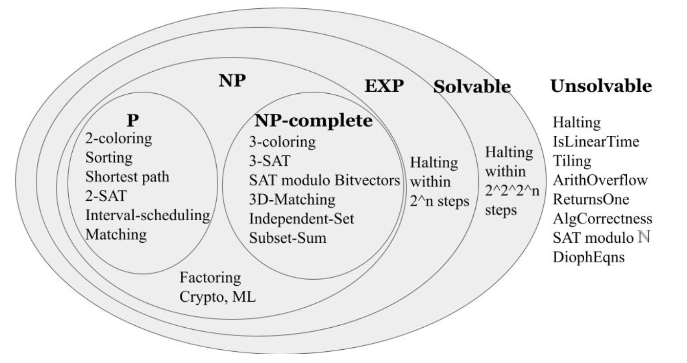
\includegraphics[width=3.5in]{figures/table.png}
        \end{minipage}

\vspace{1.5in}

\end{multicols*}
\end{document}